\documentclass[12pt,b5paper,twoside,openright]{book}
\usepackage{blindtext}
\usepackage{microtype}
\usepackage{listings}
\usepackage{color}
\usepackage{xcolor}
\usepackage{enumerate}
\usepackage{caption}
\usepackage{amsmath}
\usepackage{float}
\usepackage{algorithm}% http://ctan.org/pkg/algorithm
\usepackage{algpseudocode}% http://ctan.org/pkg/algorithmicx
\usepackage{graphicx}

\renewcommand{\chaptername}{Bab}
\renewcommand{\contentsname}{Daftar Isi}
\renewcommand{\listfigurename}{Daftar Gambar}
\renewcommand{\listtablename}{Daftar Tabel}
\renewcommand{\figurename}{Gambar}
\renewcommand{\tablename}{Tabel}
\usepackage{imakeidx}
\makeindex[columns=2, title=Indek,options= -s example_style.ist]

\usepackage{fancyhdr}
\pagestyle{fancy}
\fancyhf{}
\fancyhead[LE]{\rightmark}
\fancyhead[RO]{\leftmark}
\fancyfoot[LE,RO]{\thepage}
 
\renewcommand{\headrulewidth}{1pt}
\renewcommand{\footrulewidth}{1pt}
\pagenumbering{roman}


\usepackage{draftwatermark}
\SetWatermarkText{DRAFT}
\SetWatermarkScale{5}
\SetWatermarkColor[gray]{0.95}
 

\begin{document}
%% for code snippet
\definecolor{dkgreen}{rgb}{0,0.6,0}
\definecolor{gray}{rgb}{0.5,0.5,0.5}
\definecolor{mauve}{rgb}{0.58,0,0.82}
\lstset{frame=tb,
  language=Java,
  aboveskip=3mm,
  belowskip=3mm,
  showstringspaces=false,
  columns=flexible,
  basicstyle={\small\ttfamily},
  numbers=left,
  numberstyle=\small\ttfamily\color{black},
  keywordstyle=\color{blue},
  commentstyle=\color{dkgreen},
  stringstyle=\color{mauve},
  breaklines=true,
  breakatwhitespace=true,
  tabsize=3
}

\title{{ Bagaiamana Berfikir Seperti Imuwan Komputer}}
\author{Allen Downey \\
	Diterjemahkan oleh Tim Buku Prodase - Universitas Telkom}

\date{}

\maketitle
\newpage

\frontmatter
\tableofcontents
\addcontentsline{toc}{chapter}{Daftar Tabel}
\listoftables
\addcontentsline{toc}{chapter}{Daftar Gambar}
\listoffigures


\mainmatter
%%%%%%%%%%%%%%%%ISI BUKU%%%%%%%%%%%%%%%%%%%%%%%
\chapter{Cara Program}

Tujuan dari buku ini adalah mengajarkan kepada kamu bagaimana berfikir seperti seorang ilmuan komputer. Saya sangat suka bagaimana seorang ilmuan komputer berfikir karena mereka menggabungkan aspek-aspek terbaik dari ilmu Matematika, ilmu Teknik, dan ilmu pengetahuan alam. Sebagaimana halnya Matematikawan, ilmuan komputer menggunakan bahasa formal untuk menyatakan ide khususnya yang berkenaan dengan komputasi. Seperti Insinyur(\textit{Engineer}), ilmuan komputer juga merancang sesuatu, merangkai beberapa komponen kedalam sebuah sistem dan mengeveluasi kelebihan dan kekurangan dari berbagai alternatif solusi. Mirip dengan ilmuan pada umumnya, para ilmuan komputer melakukan observasi tingkah laku dari sistem yang kompleks, membentuk beberap hipotesis dan menguji prediksi yang mereka buat.

Satu-satunya keahlian yang paling penting bagi seorang ilmuan komputer adalah keahlian dalam memecahkan masalah (\textit{problem-solving}). Yang saya maksudkan dengan kemampuan memecahkan masalah adalah kemampuan mereka dalam melakukan formulasi masalah, berfikir secara kreatif mengenai solusi dari masalah yang telah diformulasikan dan mengekspresikan sebuah solusi secara jelas dan akurat.  Dan ternyata proses yang kamu lalui ketika belajar program komputer  adalah sebuah kesempatan yang istimewa  dalam berlatih keahlian memecahkan masalah. Itu kenapa judul dari bab ini adalah "Cara Program".

Pada satu sisi kamu akan belajar pemrograman, yang mana merupkah keahlian yang sangat penting. Disisi lainya, kamu akan menggunakan pemrograman sebagai sarana untuk belajar 

\section{Apa itu bahasa pemrograman?}

Bahasa pemrograman yang akan kamu \textbf pelajari adalah Java, yang termasuk sebuah bahasa pemrograman yang relatif baru (Dirilis pertama kali oleh Sun Microsystem pada may 1995). Java adalah salah satu contoh dari bahasa pemrograman level tinggi (\textit{high-level language}); bahasa pemrograman lain yang juga termasuk kategori bahasa pemrograman level tinggi adalah bahasa Python, C atau C++ dan Perl.

Selain istilah bahasa pemrograman level tinggi, terdapat juga istilah bahasa pemrograman level rendah (\textit{low level languages}) dan terkadang dikenal juga dengan istilah bahasa mesin atau bahasa \textit{assembly}. Pada kenyataanya, komputer hanya bisa memahami bahasa pemrograman level rendah. Oleh sebab itu, sebuah program yang ditulis menggunakan bahasa level tinggi harus diterjemahkan terlebih dahulu ke bentuk bahasa level rendah sebelum program tersebut dijalankan. Proses penterjemahan ini membutuhkan waktu sebelum bisa dijalankan oleh komputer, hal ini menjadi salah satu kekurangan dari bahasa pemrograman level tinggi.

Keunggulan dari bahasa  level-tinggi cukup banyak jika dibandingkan dengan kekuranganna. Pertama, jauh lebih mudah untuk membuat program dengan menggunakan bahasa level-tinggi; waktu yang dibutuhkan untuk menuliskan program jauh lebih singkat, penulisannya juga jauh lebih pendek dan mudah dibaca jika dibandingkan dengan bahasa level-rendah. Keuntungan yang kedua adalah portabilitas dalam menjalankannya diberbagai macam arsitektur komputer dengan tanpa modifikasi. Berbeda halnya dengan program yang ditulis dengan bahasa level-rendah yang hanya bisa dijalankan di komputer tertentu, sehingga perlu dimodifikasi jika ingin dijalankan pada komputer dengan arsitektur yang berbeda.

Oleh karena kelebiha-kelebihan tersebut, maka hampir semua program ditulis dengan menggunakan bahasa pemrograman level-tinggi. Bahasa level-rendah hanya digunakan untuk membuat program-program tertentu saja yang jumlahnya juga sedikit.

Terdapat dua cara untuk menterjemahkan sebuah program; \textbf{interpretasi} (\textit{interpreting}) dan \textbf{kompilasi} (\textit{compiling}). Sebuah \textit{interpreter} adalah sebuah program yang membaca sebuah program level-tinggi dan melakukan apa yang diminta oleh program tersebut. Sebagai akibatnya, interpreter akan menterjemahkan program baris demi baris
Sementara \textit{complier} adalah sebuah program yang membaca sebuah program level-tinggi dan menterjemahkan keseluruhan program secara langsung, sebelum menjalankan perintah apa pun dari program tersebut. Sering kali, kamu akan melakukan proses kompilasi secara terpisah terlebih dahulu, kemudian baru  menjalankan program. Pada kasus ini, program level-tinggi disebut dengan istilah kode sumber (\textit{source code}) dan program yang telah diterjemahkan disebut dengan istilah kode objek (\textit{object code}) atau \textit{executable}.


 %%merujuk ke berkas Bab-1.tex
\chapter{Pengkondisian dan Rekursi}

\section{Operator Modulus}

Operator modulus bekerja pada bilangan bulat (dan ekspresi integer) dimana hasilnya adalah hasil dari pembagian antara operan (bilangan) pertama dan operan kedua. Dalam Java, simbol dari operator modulus adalah tanda persen (\%). Untuk sintaksnya sama seperti operator lainnya :
\par
1. \textcolor{blue}{int} hasilBagi = 7 / 3;
\par
2. \textcolor{blue}{int} sisaBagi = 7 \% 3;
\newline
\newline
Operator pertama adalah pembagian bilangan bulat dengan hasil 2. Sedangkan operator kedua adalah operator modulus yang menghasilkan 7 sisa bagi dari 2 yaitu 1
\newline
\newline
Operator modulus tenyata sangat mengejutkan dan sangat berguna. Misalkan, kamu dapat memeriksa apakah suatu angka akan habis jika dibagi angka lain: jika x \% y adalah nol, maka x habis dibagi y.
\newline
\newline
Dan juga anda dapat menggunakan operator modulus untuk mengekstrak digit paling kanan dari atau digit sebuah nomor. Misalnya, x \% 100 menghasilkan digit paling kanan dari x (dalam basis 10). Demikian pula x \% 100 akan menghasilkan dua digit terakhir dari x


\section{Eksekusi Pengkondisian}
Untuk menulis program yang berguna, kita hampir selalu perlu untuk memeriksa kondisi dan mengubah perilaku program yang sesuai. Pernyataan bersyarat memberikan kita kemampuan untuk melakukan ini. Bentuk sederhananya adalah jika pernyataan : 
\par
\textcolor{blue}{if} (x \textgreater 0) \{
\par

System.out.println("x adalah bilangan positif");
\par
\}
\newline
\newline
Ekspresi dalam kurung "\textcolor{blue}{if} (x \textgreater 0)" disebut kondisi. Jika benar, maka pernyataan dalam kurung dijalankan. Jika kondisi ini salah, tidak ada yang terjadi.
\newline
\newline
Kondisi dapat berisi banyak operator perbandingan, terkadang disebut \textbf{Operator Relasional}
\newline
\newline
x == y \textcolor{green}{// x sama dengan y}
\newline
x != y \textcolor{green}{// x tidak sama dengan y}
\newline
x \textgreater y \textcolor{green}{// x lebih besar daripada y}
\newline
x \textless y \textcolor{green}{// x is lebih kecil daripada y}
\newline
x \textgreater= y \textcolor{green}{// x lebih besar atau sama dengan y}
\newline
x \textless= y \textcolor{green}{// x lebih kecil atau sama dengan y}
\newline
\newline
Meskipun operasi ini familiar, sintaks pada java menggunakan simbol matematika yang sedikit berbeda seperti =, 6= dan \textless=. Kesalahan yang sering dilakukan adalah menggunakan satu sama dengan (=) untuk membandingkan nilai bukan menggunakan dobel sama dengan (==). Ingat bahwa  = adalah operator penugasan, dan == adalah operator perbandingan.
\newline
\newline
Kedua operan yang dibandingkan harus memiliki tipe data yang sama. Misal, anda hanya bisa membandingkan \textcolor{blue}{int} ke \textcolor{blue}{int} dan \textcolor{blue}{double} ke \textcolor{blue}{double}.
\newline
Operator == dan != juga bekerja pada tipe data String, tetapi mereka tidak melakukan seperti apa yang anda ekspektasikan. Dan operator relasional yang lain secara keseluruhan tidak melakukan apa apa. Kita akan mempelajari bagaimana cara membandingkan string pada \textbf{Bagian 8.10.}
\newline
\section{Eksekusi Alternatif}
Bentuk kedua dari eksekusi pengkondisian adalah eksekusi alternatif, dimana ada dua kemungkinan, dan kondisi menentukan bagian mana yang akan dieksekusi. Sintaksnya seperti :
\par
\textcolor{blue}{if} (x\%2 == 0) \{
\par
System.out.println(\textcolor{orange}{"x adalah bilangan genap"});
\par
\} \textcolor{blue}{else} \{
\par
System.out.println(\textcolor{orange}{"x adalah bilangan genap"});
\par
\}
\newline
Jika sisa bagi dari x dibagi dengan 2 adalah 0, maka kita tahu bahwa x adalah bilangan genap, dan kode ini berguna untuk mencetak pernyataan tersebut. Jika kondisi salah maka peryataan kedua yang dicetak yaitu x adalah bilangan ganjil. Karena kondisi harus benar atau salah, maka hanya tepat satu alternatif yang akan dieksekusi.
\newline
Sebagai sampingan jika anda sering memeriksa paritas (pemerataan atau keanehan) nomor, maka anda dapat "membungkus" kode ini ke dalam sebuah method, sebagai berikut:
\par
\textcolor{blue}{public static void} printParity(\textcolor{blue}{int} x) \{
\par
\textcolor{blue}{if} (x\%2 == 0) \{
\par
System.out.println(\textcolor{orange}{"x adalah bilangan genap"});
\par
\} \textcolor{blue}{else} \{
\par
System.out.println(\textcolor{orange}{"x adalah bilangan genap"});
\par
\}
\par
\}
\newline
Sekarang anda memiliki method yang bernama printParity yang berfungsi untuk mencetak pesan yang sesuai untuk setiap bilangan bulat yang anda berikan. Dalam method utama, anda dapat memanggil method printParity dengan cara :
\newline
\par
printParity(17);
\newline
\newline
Selalu ingat ketika anda memanggil sebuah method, tidak perlu mendeklarasikan argumen. Karena java dapat mengetahui jenis tipe data mereka. Dan anda juga harus dapat menahan godaan untuk menulis hal-hal seperti :
\par
\textcolor{blue}{int} number = 17;
\par
printParity(\textcolor{blue}{int} number); \textcolor{green}{// WRONG!!!}
\section{Kondisi Berantai}
Terkadang anda  ingin memeriksa sejumlah kondisi terkait dan memilih salah satu dari beberapa tindakan. Salah satu cara untuk melakukan ini adalah dengan merantaikan antara if dan elsenya:
\par
\textcolor{blue}{if} (x \textgreater 0) \{
\par
System.out.println("x adalah bilangan positif");
\par
\} \textcolor{blue}{else if} (x \textless 0)\{
\par
System.out.println("x adalah negatif  positif");
\par
\} \textcolor{blue}{else} \{
System.out.println("x adalah nol");
\}
\newline
\newline
Rantai ini bisa sepanjang yang anda inginkan, meskipun bisa sulit untuk dibaca. Salah satu cara untuk membuat mereka lebih mudah dibaca adalah dengan menggunakan penulisan standar dengan lekukan, seperti yang ditunjukkan dalam contoh ini. Jika Anda menyimpan semua pernyataan dengan penulisan standar, maka akan meminimalisir kesalahan penulisan sintaks dan error serta lebih mudah untuk menemukan mereka jika anda melakukannya.

\section{Kondisi Bersarang}
Selain dirantaikan, kondisi juga dapat disarangkan antara satu kondisi dengan kondisi yang lain. Kita dapat menuliskan contoh dari kondisi bersarang sebagai berikut:
\par
\textcolor{blue}{if} (x \textgreater 0) \{
\par
System.out.println("x adalah bilangan positif");
\par
\} \textcolor{blue}{else} \{
\textcolor{blue}{if}(x \textless 0) \{
\par
System.out.println("x adalah negatif  positif");
\par
\} \textcolor{blue}{else} \{
System.out.println("x adalah nol");
\}
\}
\newline
\newline
Sekarang terdapat terdapat kondisi dengan dua cabang, Cabang yang pertama berisi perintah untuk mencetak pernyataan sederhana, tetapi cabang yang kedua berisi pernyataan kondisi yang lain yang memiliki dua cabang. Kedua cabang kondisi tersebut sama sama untuk mencetak pernyataan sederhana. Tetapi mereka adalah pernyataan kondisi yang benar.
\newline
Lekukan membantu membuat struktur yang jelas, namun demikian, kondisi bersarang sulit jika dibaca dengan sangat cepat. Maka hindari mereka sebisa mungkin.
\newline
Di sisi lain, struktur bersarang semacam ini adalah hal yang umum, dan kita pasti akan menemuinya lagi, sehingga anda dapat lebih baik untuk menggunakannya.

\section{Pernyataan Pengembalian}
Pernyataan pengembalian memungkinkan anda untuk mengakhiri eksekusi method sebelum Anda mencapai akhir. Salah satu alasan untuk menggunakannya adalah jika Anda mendeteksi kesalahan kondisi:
\newline
\par
\textcolor{blue}{public static void} printLogarithm(\textcolor{blue}{double} x) \{
\par
\textcolor{blue}{if} (x \textless= 0.0) \{
\par
System.out.println(\textcolor{orange}{"Tolong masukkan bilangan positif saja"});
\par
\textcolor{blue}{return};
\par
\}
\par
\textcolor{blue}{double} result = Math.log(x);
\par
System.out.println(\textcolor{orange}{"Hasil log dari x adalah "} + result);
\par
\}
\newline
\newline
Baris kode diatas mendefinisikan sebuah method printLogarithm dengan parameter berupa tipe data double yang bernama x. Method ini berfungsi untuk memeriksa apakah x kurang dari atau sama dengan nol, jika benar maka method ini akan mencetak pesan error dan menggunakan return untuk keluar dari method. Aliran dari eksekusi, segera mengembalikan segera kembali ke pemanggil dan sisa baris di method tidak dieksekusi.

\section{Tipe Konversi}
Anda mungkin bertanya-tanya bagaimana ekspresi seperti \textbf{"Hasil dari log x adalah" + result} tidak error. Hal ini karena salah satu operan bertipe \textbf{String} dan yang lainnya bertipe \textbf{double}. Inilah salah satu keunggulan dari Java yaitu, secara otomatis mengkonversi operan yang bertipe double menjadi String sebelum ia melakukan penggabungan antar string. 
\newline
Setiap kali Anda mencoba untuk "menambahkan" dua ekspresi, jika salah satu dari mereka adalah \textbf{String}, Java mengubah String lain, kemudian melakukan penggabungan string (concatination). Menurut anda apa yang akan terjadi jika anda melakukan operasi antara sebuah integer dan sebuah nilai floating-point?

\section{Rekursi}
Seperti yang saya sebutkan dalam bab terakhir bahwa salah satu method untuk boleh memanggil method yang lain, dan kita juga telah melihat beberapa contohnya. Saya tidak menyebutkan bahwa sebuah metode boleh untuk memanggil dirinya sendiri. Ini mungkin tidak jelas mengapa itu adalah hal yang baik, tapi ternyata menjadi salah satu hal yang paling ajaib dan menarik yang dapat dilakukan sebuah program .
\newline
Sebagai contoh, lihat method berikut:
\par
\textcolor{blue}{public static void} countdown(\textcolor{blue}{int} n) \{
\par
\textcolor{blue}{if} (n ==  0) \{
\par
System.out.println(\textcolor{orange}{"Waktu Habis!"});
\par
	\} \textcolor{blue}{else} \{
\par	
	System.out.println(n);
\par	
	countdown(n-1);
\par	
\}
\par
\}
\newline
Nama method ini adalah countdown dan dibutuhkan satu bilangan bulat sebagai parameter. Jika parameternya nol, maka mencetak kata "Waktu Habis!" Jika tidak, akan mencetak nomor dan kemudian memanggil method countdown sendiri dengan \textbf{n - 1} sebagai argumen. Apa yang terjadi jika kita memanggil metode ini pada method utama seperti ini:
\newline
\par
countdown (3);
\newline
\newline
Eksekusi method countdown akan dimulai dengan n = 3, karena n tidak nol, maka akan mencetak nilai 3, dan kemudian memanggil method countdown kembali...
\newline
\newline
Eksekusi method countdown akan dimulai dengan n = 2, karena n tidak nol, maka akan mencetak nilai 2, dan kemudian memanggil method countdown kembali...
\newline
\newline
Eksekusi method countdown akan dimulai dengan n = 1, karena n tidak nol, maka akan mencetak nilai 1, dan kemudian memanggil method countdown kembali...
\newline
\newline
Eksekusi method countdown akan dimulai dengan n = 0, karena n adalah nol, maka akan mencetak "Waktu Habis!", dan mengembalikan nilai \textbf{n}...
\newline
\newline
Method countdown ini menghasilkan \textbf{n=1}
\newline
\newline
Method countdown ini menghasilkan \textbf{n=2}
\newline
\newline
Method countdown ini menghasilkan \textbf{n=3}
\newline
\newline
Kemudian anda kembali pada method utama, maka output secara keseluruhannya adalah :
\newline
3
\newline
2
\newline
1
\newline
Waktu Habis!
\newline
Sebagai contoh kedua, mari kita lihat lagi di method newLine dan
threeline.
\par
\textcolor{blue}{public static void} newLine() \{
\par
	System.out.println (\textcolor{orange}{""});
	\par
\}
\newline
	\par
\textcolor{blue}{public static void} threeLine() \{
		\par
	newLine(); 
		\par
	newLine(); 
		\par
	newLine();
		\par
\}
\newline
\newline
Pekerjaan ini tidak akan banyak membantu jika kita ingin mencetak 2 atau 106 baris. Sebuah alternatif yang lebih baik adalah:
\par
\textcolor{blue}{public static void} nLines(\textcolor{blue}{int} n) \{
\par
	if (n \textless 0) \{
	\par
		System.out.println (\textcolor{orange}{""});
		\par
		nLines (n-1);
		\par
	\}
	\par
\}
\newline
\newline
Program ini mirip dengan countdown; selama n lebih besar dari nol, ia akan mencetak baris baru dan kemudian memanggil dirinya dengan argumen \textbf{n-1} untuk mencetak baris tambahan. Jumlah dari baris yang bisa dicetak adalah 1 + (n-1).
\newline
\newline
Ketika metode memanggil dirinya sendiri disebut \textbf{rekursi}, dan metodenya adalah \textbf{rekursif}

\section{Diagram Stack untuk Method Rekursif}
 Dalam bab sebelumnya kita menggunakan diagram stack untuk mewakili negara dari sebuah program selama pemanggilan method. Diagram yang sama dapat mempermudah untuk menafsirkan metode rekursif. 
 \newline
 Ingat bahwa setiap kali sebuah method dipanggil itu menciptakan kerangka baru yang berisi versi baru dari parameter method dan variabel. 
 \newline
  \newline
 Gambar berikut adalah diagram stack untuk method countdown, dengan n = 3:
 \par
 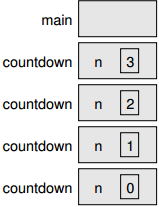
\includegraphics{diagram}
 \newline
 \newline
 Ada satu frame untuk utama dan empat frame untuk method countdown, masing-masing dengan nilai yang berbeda untuk parameter n. Pada bagian paling bawah tumpukan, terdapat method countdown dengan n = 0, tumpukan ini disebut \textbf{base case}. Hal ini tidak membuat panggilan rekursif, sehingga tidak ada lagi frame untuk menjalankan method countdown. Frame untuk utama adalah kosong karena utama tidak memiliki parameter atau variabel.
 \newline
 \newline
 \section{Rangkuman}
 \textbf{Modulus}: Sebuah operator yang bekerja pada bilangan bulat dan menghasilkan sisa bagi ketika satu nomor dibagi dengan yang lain. Di java modulus dilambangkan dengan tanda persen (\%).
  \newline
    \newline
 \textbf{Kondisional}: Sebuah blok pernyataan yang mungkin atau mungkin tidak akan dieksekusi tergantung pada beberapa kondisi.
  \newline
    \newline
 \textbf{Chaining}: Sebuah cara untuk menggabungkan beberapa pernyataan kondisional secara berurutan.
  \newline
    \newline
\textbf{Nesting}: Menempatkan pernyataan kondisional dalam salah satu atau kedua cabang pernyataan kondisional lain.
 \newline
   \newline
 \textbf{Typecast}: Sebuah operator yang mengkonversi dari satu jenis tipe data ke tipe data yang lain. Di java biasanya nama tipe data berada dalam tanda kurung, seperti (int).
  \newline
  \newline
 \textbf{Rekursi}: Proses memanggil metode yang sama yang sedang anda eksekusi.
 \newline
 \newline
 \textbf{Base Case}: Sebuah kondisi yang menyebabkan metode rekursif tidak untuk membuat panggilan rekursif.
\newline
\newline

\section{Latihan}
\textbf{Latihan 4.1.} Gambarkan diagram stack yang menunjukkan keadaan dari program dalam Bagian 4.8 setelah method utama memanggil nLines dengan parameter n = 4, tepat sebelum pemanggilan terakhir nLines dikembalikan.
\newline
\textbf{Latihan 4.2.} Latihan ini adalah meninjau aliran eksekusi melalui program dengan beberapa metode. Baca kode berikut dan menjawab pertanyaan-pertanyaan di bawah ini.
\par
public class Buzz \{
	\par
	public static void baffle(String blimp) \{
		\par
		System.out.println(blimp);
		\par
		zippo("ping", -5);
		\par
	\}
	\newline
	\par
	public static void zippo(String quince, int flag)\{
		\par
		if (flag \textless 0) \{
			\par
			System.out.println(quince + " zoop");
			\par
		\} else \{
		\par
		System.out.println("ik");
		\par
		baffle(quince);
		\par
		System.out.println("boo-wa-ha-ha");
		\par
	\}
			\par
\}
\newline
\newline
public static void main(String[] args) \{
	\par
	zippo("rattle", 13);
	\par
\}
\par
\}
\newline
\newline
1. Tuliskan nomor 1 di sebelah pernyataan pertama dari program ini yang akan dieksekusi. Hati-hati untuk membedakan hal-hal yang pernyataan dari hal-hal yang tidak.
2. Tuliskan nomor 2 di sebelah pernyataan kedua, dan seterusnya sampai akhir program. Jika pernyataan dieksekusi lebih dari sekali, itu mungkin berakhir dengan lebih dari satu nomor sebelahnya.
3. Berapa nilai dari parameter \textbf{blimp} saat \textbf{baffle} akan dipanggil?
4. Apa output dari program ini?
\newline
\newline
\textbf{Latihan 4.3.} Lirik pertama dari lagu "99 Botol Bir" adalah:
\newline
\par
99 bottles of beer on the wall, 99 bottles of beer, ya’ take one
down, ya’ pass it around, 98 bottles of beer on the wall.
\newline
\newline
Lirik berikutnya adalah identik kecuali bahwa jumlah botol semakin kecil oleh salah satu di setiap lirik, sampai lirik terakhir:
\newline
\par
No bottles of beer on the wall, no bottles of beer, ya’ can’t take one down, ya’ can’t pass it around, ’cause there are no more
bottles of beer on the wall!
\newline
\newline
Dan kemudian lagu (akhirnya) berakhir.
\newline
\newline
Tulis sebuah program yang mencetak seluruh lirik "99 Botol bir." Program harus mencakup metode rekursif yang melakukan bagian yang sulit, tapi anda mungkin ingin menulis method tambahan untuk memisahkan fungsi utama program.
\newline
\newline
Ketika Anda mengembangkan kode Anda, uji dengan sejumlah lirik kecil, seperti "3 Botol Bir. "
\newline
\newline
Tujuan dari latihan ini adalah untuk mengambil masalah dan memecahnya menjadi lebih kecil masalah, dan untuk memecahkan masalah yang lebih kecil dengan menulis metode sederhana.
\newline
\newline
\textbf{Latihan 4.4.} Apa output dari program ini?
\newline
\par
public class Narf \{
\par
	public static void zoop(String fred, int bob) \{
	\par
		System.out.println(fred);
		\par
		if (bob == 5) \{
		\par
			ping("not ");
			\par
		\} else \{
		\par
		System.out.println("!");
		\par
	\}
	\par
\}
\newline
\par
public static void main(String[] args) \{
\par
	int bizz = 5;
	\par
	int buzz = 2;
	\par
	zoop("just for", bizz);
	\par
	clink(2*buzz);
	\par
\}
\newline
\par
public static void clink(int fork) \{
\par
	System.out.print("It's ");
	\par
	zoop("breakfast ", fork) ;
	\par
\}
\newline
\par

public static void ping(String strangStrung) \{
	\par
	System.out.println("any " + strangStrung + "more ");
	\par
\}
\par
\}
\newline
\newline
\textbf{Latihan 4.5.} Fermat terakhir Teorema mengatakan bahwa tidak ada bilangan bulat a, b, dan c sehingga:
\newline
an + bn = cn
\newline
\newline
kecuali dalam kasus ketika n = 2.
\newline
\newline
Tulis sebuah metode checkFermat bernama yang mengambil empat bilangan bulat sebagai parameter a, b, c dan n. Lalu periksa untuk melihat apakah teorema Fermat benar. Jika n lebih besar dari 2 dan ternyata benar bahwa an + bn = cn, dan program harus mencetak "Teori Fermat adalah salah!" Jika tidak program harus mencetak "Tidak, yang tidak bekerja. "
\newline
Anda harus mengasumsikan bahwa ada method raiseToPow bernama yang mengambil dua bilangan bulat sebagai argumen dan memunculkan argumen pertama untuk kekuatan kedua. Sebagai contoh:
\newline
\newline
int x = raiseToPow (2, 3);
\newline
\newline
maka nilai 8 untuk x, karena $2^3$ = 8
 %%merujuk ke berkas Bab-4.tex
%%%%%%%%%%%%%%%%%%%%%%%%%%%%%%%%%%%%%%%%%%%%%%%%%%%%%%%
\backmatter
%\include{glossary}

\printindex
\end{document}